\section{Opening and Viewing a Data Package} \label{sec:viewing}

Existing data packages, which consist of metadata and (optionally) the
data set described by the metadata, are easily opened and viewed in
Morpho. Whether your data package is stored locally, on the network, or
both, you can easily open it with Morpho's Data Package viewer. If you
have permission to access the data, you can also open data packages
created by other scientists. 

\subsection{Opening Data Packages}

To open a data package that you have created, use one of the following
techniques:

\begin{itemize}
  \setlength{\parskip}{1pt}
  \item click the ``Open an existing data package...'' on the ``Work
    with your data'' panel on the Main Morpho screen,
  \item select the ``Open'' menu item from the File menu,
  \item click the 
\includegraphics[scale=0.7]{images/button-open.png}
  icon in the Toolbar.
\end{itemize}

You will then see a listing of the available data packages
(\autoref{fig:open-dp}). Available data packages include those which you
previously created using the current profile and/or under the current
KNB username, along with a fictitious sample data package included with
Morpho -- ``Population sampling data for zooplankton in the Great Lakes,
2000''.

\begin{figure}
  \centering
    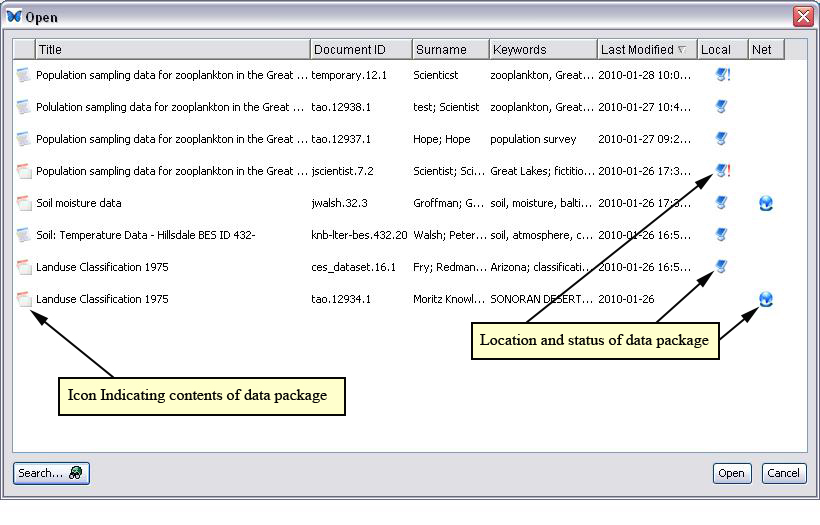
\includegraphics[width=0.7\textwidth]{images/open-dp.jpg}
  \caption{An example listing of available data packages displayed in
    Morpho's Open screen.}
  \label{fig:open-dp}
\end{figure}

The icons in the first column of the Open Data Package screen tell you
if the package contains:
\begin{itemize}
  \parskip 3pt
  \itemsep 0pt
  \item[] 
\includegraphics[scale=0.7]{images/indicator-hasdata.png}
    Data and documentation
  \item[] 
\includegraphics[scale=0.7]{images/indicator-hasnodata.png}
	Documentation only 
\end{itemize}

Icons in the last two columns indicate the location and status of the
package:
\begin{itemize}
  \parskip 3pt
  \itemsep 0pt
  \item[] 
\includegraphics[scale=0.7]{images/indicator-dp-local.png}
  Local data package
  \item[] 
\includegraphics[scale=0.7]{images/indicator-dp-incomplete.png}
  Saved incomplete data package
  \item[] 
\includegraphics[scale=0.7]{images/indicator-dp-network.png}
  Network data package
  \item[] 
\includegraphics[scale=0.7]{images/indicator-dp-recovered.png}
  Recovered incomplete data package
\end{itemize}

For more information about saved and recovered incomplete data package,
please see \autoref{sec:dp-saveforlater} and
\autoref{sec:dp-recover}.

Select a data package to open (or open the fictitious sample package
``Population sampling data for zooplankton in the Great Lakes, 2000'').
To open a selected package, click the ``Open'' button located at the
bottom right of the screen, or double-click the selected data package,
or right-click the data package and select ``Open Package''
(\autoref{fig:menu-dp-rightclick}). You can also open an earlier version
of the data package (if any exist) by right-clicking the package and
selecting ``Open Previous Version.'' Note that one or more previous
versions of the data package may be unavailable, for example, a version
saved only locally on a different computer. The Refresh command updates
the listing of available packages.

\begin{figure}
  \centering
    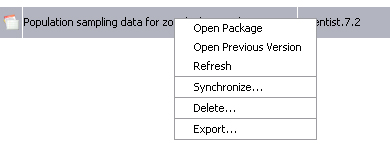
\includegraphics[width=0.7\textwidth]{images/menu-dp-rightclick.jpg}
  \caption{Right-click a data package to open an action menu.}
  \label{fig:menu-dp-rightclick}
\end{figure}

\begin{shaded}
  \textbf{NOTE} Morpho automatically displays data packages stored in
  earlier versions of EML (e.g., 2.0 or Beta 6) as EML 2.0. If a package
  does not use the latest EML format, Morpho will prompt users to
  transform the EML to the latest version. If you choose to transform
  the EML, you will need to save the data package to preserve the
  changes, at which time the revision number of the document will be
  incremented. If the updated EML document is invalid (e.g., a required
  metadata field is blank), a correction wizard opens to allow users to
  fix the problem. For more information, please see
  \autoref{sec:upgrading-eml}.
\end{shaded}

\subsubsection*{Opening a Shared Data Package}

To locate and view data packages other than those you have created, use
the \hyperref[sec:searching]{Search} feature, which is described later
in this guide. You can only open and view data packages for which you
have been granted permission. If you do not have permission to open a
data package, it will not appear in your search results. 

\paragraph{NOTE}
If you are not logged in to the KNB, but have network access, the only
network data packages that will appear in your search are those that
have ``public'' access privileges. To view additional data sets from the
KNB network, log in to the network.

\subsection{Viewing a Data Package: The Data Package Interface}

When you open a data package, Morpho displays it in the Data Package
interface (\autoref{fig:viewer-table-main}). The Data Package interface
contains the standard Menu bar and Toolbar as well as three panels: the
\nameref{sec:panel-dp-doc}, the \nameref{sec:panel-table}, and the
\nameref{sec:panel-table-doc}.

\begin{figure}
  \centering
    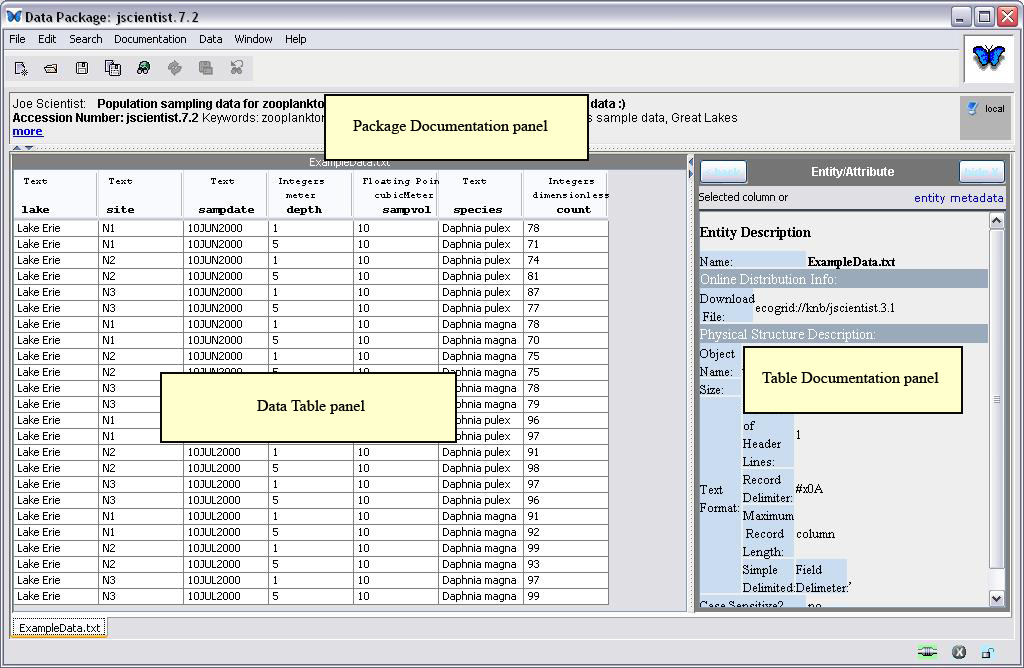
\includegraphics[width=0.7\textwidth]{images/viewer-table-main.jpg}
  \caption{Viewing a data package in Morpho's Data Package interface.}
  \label{fig:viewer-table-main}
\end{figure}

\subsubsection{Package Documentation panel} \label{sec:panel-dp-doc}

The Package Documentation panel contains a brief ``citation-style''
summary of the data package: its title, description, usage information,
etc. The icons on the right side of the panel indicate whether the
package is located on the local machine, on the network, or both
(\autoref{fig:viewer-table-top}). No icons will appear if the data
package has not yet been saved, or has been modified since it was last
saved.
 
\begin{figure}
  \centering
    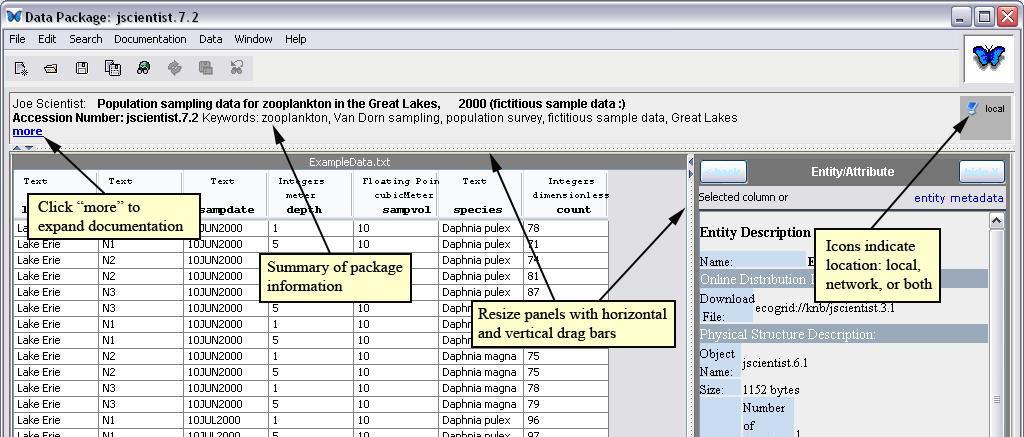
\includegraphics[width=0.7\textwidth]{images/viewer-table-top.jpg}
  \caption{The Data Package panel.}
  \label{fig:viewer-table-top}
\end{figure}

The Package Documentation panel can be expanded to reveal additional
documentation, either by dragging the horizontal drag bar, or by
clicking the ``more'' link (\autoref{fig:viewer-metadata-options}).

\begin{figure}
  \centering
    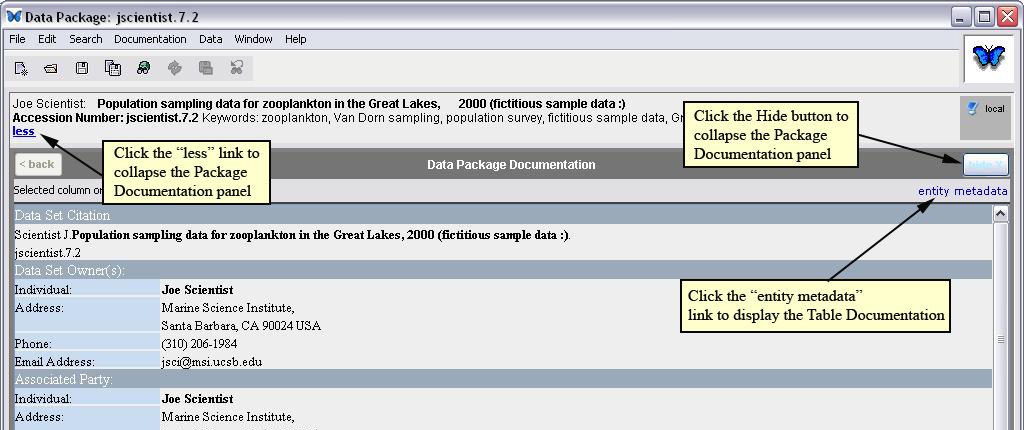
\includegraphics[width=0.7\textwidth]{images/viewer-metadata-options.jpg}
  \caption{The Package Documentation panel after it has been expanded.}
  \label{fig:viewer-metadata-options}
\end{figure}


To collapse the Package Documentation panel:
\begin{itemize}
  \setlength{\parskip}{1pt}
  \item click the ``less'' link 
  \item click the ``hide'' button 
  \item use the mouse to drag the divider bar from the bottom of the
    screen
  \item click the small arrow icon located on the left side of the
    divider bar 
\end{itemize}

To edit the documentation in the \hyperref[sec:edit-doc-tree]{Morpho
Editor}, click the ``Edit'' button. 

\subsubsection{Data Table panel} \label{sec:panel-table}

The Data Table panel (\autoref{fig:viewer-table-bottom}) displays
tabular data in spreadsheet form or image data (for several formats of
image entities). Use the tabs along the bottom of the Data Table panel
to select and view different data tables or image entities contained in
the data package. Use the drag bar on the right side of the panel to
collapse, expand, or change the size of the panel.

\begin{figure}
  \centering
    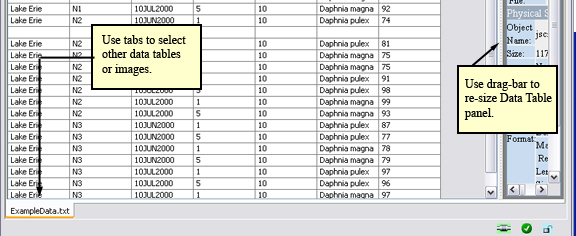
\includegraphics[width=0.7\textwidth]{images/viewer-table-bottom.jpg}
  \caption{The Data Table panel.}
  \label{fig:viewer-table-bottom}
\end{figure}

Click a table cell to edit the data directly. To save changes, use the
Save option under the File menu. To cancel all changes that have been
made to the current panel, choose ``Revert Entity to Saved Version'' under
the Edit menu. Note that it is not currently possible to undo individual
changes made to a panel. To cancel changes that have been made to ALL
data panels, select ``Revert all Entities to Saved Version'' under the
Edit menu.

Right-click the data table to display a menu that allows you to:
\begin{itemize}
  \setlength{\parskip}{1pt}
  \item sort columns 
  \item insert and delete rows 
  \item insert and delete columns 
  \item delete the entire table
  \item add new tables 
  \item add/edit documentation 
\end{itemize}

These same options are also available under the Data menu in the Menu
bar. Read more about using these tools in \autoref{sec:working-with-data}.

\subsubsection{Table Documentation panel} \label{sec:panel-table-doc}

The Table Documentation panel (\autoref{fig:viewer-table-metadata}) displays
documentation for the currently displayed table. Note that tables are
also referred to as ``entities'' in Morpho, using terminology consistent
with database management systems. Similarly, ``attributes'' refers to
table columns (also called ``variables'').

\begin{figure}
  \centering
    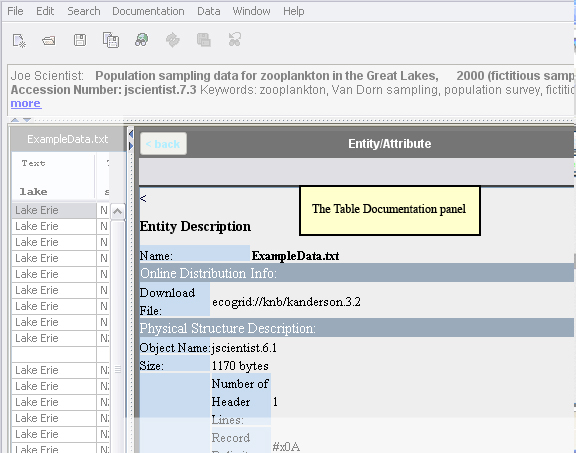
\includegraphics[width=0.7\textwidth]{images/viewer-table-metadata.jpg}
  \caption{The Table Documentation panel (expanded).}
  \label{fig:viewer-table-metadata}
\end{figure}

Click any column header in the Data Table panel to display more specific
information about the selected column in the Table Documentation panel
(\autoref{fig:viewer-column-metadata}).

Return to the table documentation by clicking the Data Table tab at the
bottom of the Data Table panel or on the ``entity metadata'' link. The
``Back'' button works like the back button in a web browser; if you have
viewed several columns of data documentation, the back button will step
back through those column descriptions before returning to the table
documentation. 

To resize the panel, drag the divider bars. Hide or fully expand the
panel by clicking the arrows on the divider bars, or by clicking the
``Hide'' button at the top-right corner. 

\begin{figure}
  \centering
    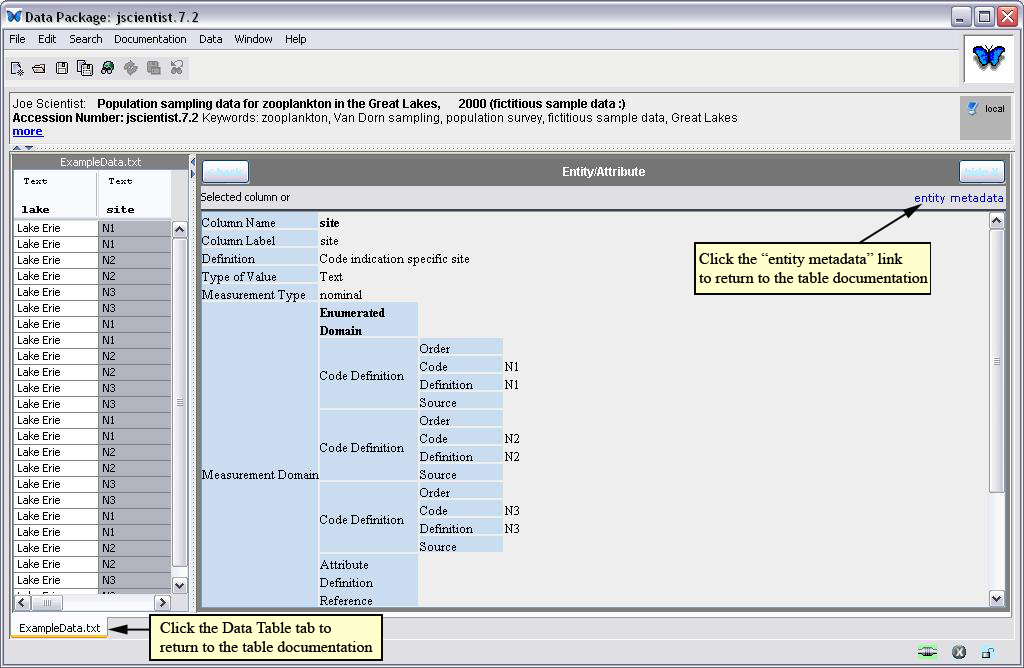
\includegraphics[width=0.7\textwidth]{images/viewer-column-metadata.jpg}
  \caption{Displaying information about a table column in the Table
    Documentation panel.}
  \label{fig:viewer-column-metadata}
\end{figure}

